%%%%%%%%%%%%%%%%%%%%%%%%%%%%%%%%%%%%%%%%%%%%%%%%%%%%%%%
%                   File: OSAmeetings.tex             %
%                  Date: 20 September 2021            %
%                                                     %
%     For preparing LaTeX manuscripts for submission  %
%       submission to Optica meetings and conferences %
%                                                     %
%       (c) 2021 Optica                               %
%%%%%%%%%%%%%%%%%%%%%%%%%%%%%%%%%%%%%%%%%%%%%%%%%%%%%%%

\documentclass[letterpaper,10pt]{article} 
%% if A4 paper needed, change letterpaper to A4

\usepackage{osameet3} %% use version 3 for proper copyright statement

%% standard packages and arguments should be modified as needed
\usepackage{amsmath,amssymb}
\usepackage[colorlinks=true,bookmarks=false,citecolor=blue,urlcolor=blue]{hyperref} %pdflatex
%\usepackage[breaklinks,colorlinks=true,bookmarks=false,citecolor=blue,urlcolor=blue]{hyperref} %latex w/dvipdf

\usepackage[english]{babel}
\newtheorem{theorem}{Theorem}
\newtheorem{corollary}{Corollary}
\newtheorem{lemma}[theorem]{Lemma}
\newtheorem{conjecture}{Conjecture}
\newtheorem{definition}{Definition}
\newtheorem{workdefinition}{Working Definition}
\newtheorem{problem}{Problem}

\usepackage{color}
\newcommand\dashto{\mathrel{
  -\mkern-6mu{\to}\mkern-20mu{\color{white}\bullet}\mkern12mu
}}

\newcommand\indep{\perp \!\!\! \perp}

\usepackage{caption}
\usepackage{subcaption}

\usepackage{tikz} 

\begin{document}

\title{Research Corral}

\author{Author name(s)}
\address{Author affiliation and full address}
\email{e-mail address}
%%Uncomment the following line to override copyright year from the default current year.
\copyrightyear{2022}


\begin{abstract}
abstract
\end{abstract}


\section{First steps on non-markovian response incentives}

% \begin{figure}
% \centering
% \begin{subfigure}{.5\textwidth}
%   \centering
%     \begin{tikzpicture}[node distance={15mm}, thick, main/.style = {draw, circle}] 
%     \node[main] (1) {$X_1$}; 
%     \node[main] (2) [below right of=1] {$D$}; 
%     \node[main] (3) [below left  of=2] {$X_2$};
%     \node[main] (4) [right of=2] {$Y$}; 
%     \color{red}\draw[->] (1) -- (2);
%     \draw[->] (3) -- (2);
%     \color{black}\draw[->] (2) -- (4);
%     \draw[dashed,<->] (3) -- (4);
%     \end{tikzpicture}
%   \caption{Direct effect of $\mathbf{X}=\{X_1,X_2\}$ on $D$}
%   \label{fig:direct}
% \end{subfigure}%
% \begin{subfigure}{.5\textwidth}
%   \centering
%     \begin{tikzpicture}[node distance={15mm}, thick, main/.style = {draw, circle}] 
%     \node[main] (1) {$X_1$}; 
%     \node[main] (2) [below right of=1] {$D$}; 
%     \node[main] (3) [below left  of=2] {$X_2$};
%     \node[main] (4) [right of=2] {$Y$}; 
%     \color{green}\draw[->] (1) -- (2);
%     \color{blue}\draw[->] (3) -- (2);
%     \color{black}\draw[->] (2) -- (4);
%     \draw[dashed,<->] (3) -- (4);
%     \end{tikzpicture}
%   \caption{Decomposition of the direct effect of $\mathbf{X}$ on $D$}
%   \label{fig:decomp}
% \end{subfigure}
% \caption{A simple example of an incentives decomposition of the direct effect of $\mathbf{X}$ on $D$, as rewarded by $Y$.}
% \label{fig:simple}
% \end{figure}

The following notation and definitions help keep consistency with the lab's existing work on both fairness\cite{r30} and CRL \cite{r57} (see Figure \ref{fig:direct} for a visual aid). In addition to the usual SCM $M=(V,U,F,P(U))$, we use $Y$ as the reward variable(s), $D\in An(Y)$ as the decision node, and $X\in An(D)$ as the sensitive attribute(s) which the decision may be unfair towards. $\mathbf{C}\subset V$ are the covariates which $D$ is allowed to observe; that is, $Pa(D)\subset \mathbf{C}$. A policy $\pi$ is a soft intervention on $D$ which respects $domain(\pi)\subset \mathbf{C}\cup \{U_D\}$, and an \emph{optimal policy} is defined as a policy $\pi$ that maximizes the sum of the expected rewards: $\mathbb{E}_\pi [\sum_{Y\in\mathbf{Y}}Y]$.
Lastly, a `fairness effect $E$' is just some element $E\in\{Cft{\text -}DE,\hspace{2mm} Cft{\text -}IE,\hspace{2mm} Cft{\text -}SE\}$.

\begin{definition}[Response Incentive]
Let $M=(V,U,F,P(U))$ be an SCM. A policy $\pi$ responds to a variable $X\in V$ if there exists some intervention $do(X=x)$ and some exogenous unit $U=u$, such that $D_x(u) \neq D(u)$. The variable $X$ has an \emph{response incentive} if all optimal policies respond to $X$.
We say a causal diagram $G$ \emph{admits} an response incentive on $X$ if it is compatible with an SCM that has an response incentive on $X$.
\end{definition}

% \begin{definition}[Response Incentive: Revised]
% Let $M=(V,U,F,P(U))$ be an SCM. A policy $\pi$ responds to a variable $X\in V$ if there exists some intervention $do(X=x)$ and some exogenous unit $U=u$, such that $D_x(u) \neq D(u)$. The variable $X$ has an \emph{response incentive} if all optimal policies respond to $X$.
% We say a causal diagram $G$ \emph{admits} an response incentive on $X$ if it is compatible with an SCM that has an response incentive on $X$.
% \end{definition}

Note that \emph{response incentive} is a binary classification of the ancestors of $D$: either a node has an response incentive, or it doesn't.
Next, the \emph{minimal reduction} of a causal graph $G$ eliminates all edges from parents of $D$ which do not have their own d-connection to $Y$.

\begin{definition}[Minimal Reduction]
The \emph{minimal reduction} $G^{min}$ of a causal diagram $G$ is the result of removing from $G$ all edges $X\rightarrow D$ satisfying $(X\indep Y | D \cup Pa(D) \setminus X)$.
\end{definition}

Intuitively, the minimal reduction breaks all non-informative links to the decision node.
The main result from \cite{everitt2021agent} we build on is a graphical criterion for classifying a node $X$ as having an response incentive.


\begin{conjecture}[Response Incentive Criterion \cite{everitt2021agent}]\label{nonmarkov}
Let $G$ be an acyclic causal diagram. Then $G$ admits a response incentive on $X\in V$ if and only if the minimal reduction $G^{min}$ has a directed path $X\dashto D$.
\end{conjecture}

\subsection{Gathering thoughts, Next steps}
\begin{itemize}
  \item the soundness portion is proved in the main text, and relies on Lemma 25 (which in turn relies on Lemmas 24, 21, ).
  \item the completeness direction is Lemma 28, which is lengthy but does not depend on any other lemmata.
  \item the so-called completeness direction says `If the graphical criteria holds, then there is a response incentive on $X$ in at least one SCM compatible with $G$'.
  \item ...I don't think the completeness direction is the one I care as much about: it says `If I say there's a response incentive then there probably is', whereas the soundess direction says `if I don't say there's a response incentive, then there definately isn't'
  \item So I think the soundness direction is the one I want more: `If the graphical condition does not hold for $X$, then $X$ does not have a response incentive for any SCM'.
\end{itemize}
First step: Just translate the soundness direction from the text (recorded below) precisely with my notation.

Second step: Pretend the supporting Lemmata (21,24,25) all generalize to the Markovian case, and attempt to generalize this portion from the text.

Backup second: if the second step fails, try just generalizing Lemmas 21, 24, and 25, in that order.

\subsection{Original Proof (Markov case)}

The \emph{if} (completeness) direction is proved in  Lemma 28 in Appendix C.2. For the soundness direction, assume that for $G$, the minimal reduction $G^{min}$ does not contain a directed path $X\dashto D$. Let $M=(G,E,\mathbf{F},\mathbf{P})$ be any SCIM compatible with $G$. Let $M^{min}=(G^{min},E,\mathbf{F},\mathbf{P})$ be $M$, but with minimal reduction $G^{min}$. By Lemma 25 in Appendix C, there exists a $G^{min}$-respecting policy $\tilde{\pi}$ that is optimal in $M$. In $M^{min}_{\tilde{\pi}}$, $X$ is causally irrelevant for $D$ so $D_x(u) = D(u)$. Furthermore, $M_{\tilde{\pi}}$ and $M^{min}_{\tilde{\pi}}$ are the same SCM, with the functions $\mathbf{F}\cup{\tilde{\pi}}$. So $D_x(u) = D(u)$ also in $M_{\tilde{\pi}}$, which means that there is an optimal policy in $M$ that does not respond to interventions on $X$ for any $\epsilon$.

\subsection{In-text portion of soundness proof, translated to my notation}

\begin{theorem}[Response Incentive Criterion \cite{everitt2021agent}]\label{markov}
Let $G$ be a Markovian causal diagram. Assume the minimal reduction $G^{min}$ does not have a directed path $X\dashto D$.
Then $G$ does not admit a response incentive on $X\in V$.
\end{theorem}

\textbf{\emph{Proof:}}
Assume that for $G$, the minimal reduction $G^{min}$ does not contain a directed path $X\dashto D$ \color{red} (perhaps needs to be stronger for non-Markovian?)\color{black}. 
Let $M$ be any SCM compatible with $G$. 
Partition $\mathbf{Pa}_D$ into the non-requisite parents $\mathbf{Pa}^{non}_D=\{W\in \mathbf{Pa}_D : (W\indep Y | D \cup Pa(D) \setminus W)\}$ and requisite parents $\mathbf{Pa}_D^{req}=\mathbf{Pa}_D\setminus\mathbf{Pa}^{non}_D$.
(Note that by definition of $G^{min}$, $\mathbf{Pa}_D^{req}$ is precisely the set of $D$'s parents in $G^{min}$).
By Lemma 25 \color{red} (requires Markovian?)\color{black}, there exists a $G^{min}$-respecting policy $\tilde{\pi}$ that is optimal in $M$. 
Let $M_{\tilde{\pi}}:=M_{\sigma_D}$ where $\sigma_D = \tilde{\pi} (D|\mathbf{Pa}^{req}_D)$.
Since $X$ is causally irrelevant in $M_{\tilde{\pi}}$, we have $D_x(u) = D(u)$. 
This means that there is an optimal policy in $M$ that does not respond to interventions on $X$ for any $U$.
\color{red} ...which I think means there's no response incentive on $X$? \color{black}

Lemma 21 is just Rule 1 of the do-calculus, which holds for Non-Markovian.

Lemma 24 is the intersection property of d-seperation, which holds for Non-Markovian.

So only Lemma 25 and the text body need to be checked.


\subsection{Ancestry is Necessary for Response Incentive}
The following theorem is probably proved somewhere already \color{red} (TODO: look) \color{black} but it was a good exercise.

\begin{theorem}[Invariance of non-descendents to interventions]\label{invariance}
Assume $X\cap An(D)=\emptyset$. Then $D_x(u)=D(u)$ for all $x\in X$, $u\in U$.
\end{theorem}

We use the following lemma:
\begin{lemma}[Invariance Inheritance]\label{inheritance}
Assume $X\cap An(D)=\emptyset$ and $Pa(D)_x(u) = Pa(D)(u)$. Then $D_x(u)=D(u)$.
\end{lemma}

\textbf{\emph{Proof of Lemma \ref{inheritance}:}}
Let $u\in U$, $x\in X$. For convienence of notation, let $Q:=Pa(D)(u)$, the value that $Pa(D)$ realizes when $U=u$.

Then
\begin{align*}
D(u)&=D_Q(u) &\text{Consistency} \\
&=D_{Q,x}(u) &\text{Exclusion Restrictions, since }X\cap Pa(D)=\emptyset \\
&= D_x(u) &\text{Exclusion Restrictions, since }Pa(D)_x(u) = Pa(D)(u)
\end{align*}

\textbf{\emph{Proof of Theorem \ref{invariance}:}}
Let $N^i$ be the set of $D$'s $i^{\text{ }th}$ grandparents; that is, $N^0=Pa(D)$, and $N^{i+1}=Pa(N^i)\setminus N^i$. Let $l$ be the largest index corresponding to a non-empty $N^i$, that is $N^l\neq \emptyset$ and $N^{l+1}=\emptyset$. (So long as $D\neq\emptyset$, $l$ exists and is unique). Note that $\{N^0,...,N^l\}$ forms a partition of $An(D)$.

We apply Lemma \ref{inheritance} inductively in reverse order: \emph{Base case:} Since for all $W\in N^l$ we have $Pa(W)=\emptyset$, we have $W(u)=W_x(u)$ trivially by Exclusion Restrictions. Thus $N^l(u)=N_x^l(u)$. \emph{Inductive step:} Assume $N^{l-k}(u)=N_x^{l-k}(u)$. Let $W\in N^{l-k-1}$. Since $Pa(W)\subset N^{l-k}$, we have that $Pa(W)_x(u)=Pa(W)(u)$, so by Lemma \ref{inheritance}, $W_x(u)=W(u)$. Thus $N^{l-k-1}(u)=N_x^{l-k-1}$.

By applying the inductive step $l-1$ times after the base case, we obtain that $D_x(u)=D(u)$ as desired.

\begin{corollary}[Necessity of Ancestry]\label{ancestry}
Let $G$ be an acyclic causal diagram which admits a response incentive on some variable $X\in V$. Then $X\in An(D)$.
\end{corollary}

The contrapositive of the corollary follows directly from Theorem \ref{invariance}, since all policies (including optimal ones) are invariant to interventions on $X$ if $X\notin An(D)$.

\subsection{Non-Markovian Soundness}

\begin{theorem}[Non-Markovian Response Incentive Criterion]\label{nonmarkov}
Let $G$ be an acyclic causal diagram. Assume the minimal reduction $G^{min}$ does not have a directed path $X\dashto D$.
Then $G$ does not admit a response incentive on $X\in V$.
\end{theorem}

\textbf{\emph{Proof:}}
Assume that for $G$, the minimal reduction $G^{min}$ does not contain a directed path $X\dashto D$.
Let $M$ be any SCM compatible with $G$. 
Partition $\mathbf{Pa}_D$ into the non-requisite parents $\mathbf{Pa}^{non}_D=\{W\in \mathbf{Pa}_D : (W\indep \mathbf{Y}_D | D \cup \mathbf{Pa}_D \setminus W)\}$ and requisite parents $\mathbf{Pa}_D^{req}=\mathbf{Pa}_D\setminus\mathbf{Pa}^{non}_D$.
(Note that by definition of $G^{min}$, $\mathbf{Pa}_D^{req}$ is precisely the set of $D$'s parents in $G^{min}$).
By Lemma 25 \color{red} (requires Markovian?)\color{black}, there exists a $G^{min}$-respecting policy $\tilde{\pi}$ that is optimal in $M$. 
Let $M_{\tilde{\pi}}:=M_{\sigma_D}$ with $\sigma_D = \tilde{\pi} (D|\mathbf{Pa}^{req}_D)$.
Since $X$ is causally irrelevant in $M_{\tilde{\pi}}$, we have $D_x(u) = D(u)$. 
This means that there exists an optimal policy intervention on $M$ that does not respond to interventions on $X$ for any $U$, so $X$ does not have a response incentive relative to the SCM $M$. 
Since $M$ was arbitrary, $G$ does not admit a response incentive on $X$.

\color{red} (All I did was translate to Elias language, no changes were required for non-markovian). \color{black}


\subsection{Lemma 25 work}

\begin{lemma}[Lemma 25 copied: Gmin-respecting optimal policy]\label{lemma25:copy}
Every single-decision SCIM $M=(G,E,F,P)$ has an optimal policy $\tilde{\pi}$ that depends only on requisite observations. In other words, $\tilde{\pi}$ is also a policy for the minimal model $M^{min}=(G^{min},E,F,P)$. We call $\tilde{\pi}$ a $G^{min}$-respecting optimal policy.
\end{lemma}

\textbf{\emph{Proof:}}
\color{red} TODO (when translate): move up defn of $\mathbf{Y}_D$. Standardize $U$ meaning utility, or find different notation. \color{black}

First partition $\mathbf{Pa}_D^G$ into the non-requisite parents $\mathbf{Pa}^{non}_D=\{W\in \mathbf{Pa}_D : (W\indep \mathbf{Y}_D | D \cup \mathbf{Pa}_D \setminus W)\}$ and requisite parents $\mathbf{Pa}_D^{req}=\mathbf{Pa}_D^G\setminus\mathbf{Pa}^{non}_D$.

Let $\pi^*$ be an optimal policy in $M$.
To construct a $G^{min}$-respecting version $\tilde{\pi}$, select any value $\mathbf{\tilde{pa}}^{non}_D \in dom(\mathbf{Pa}^{non}_D)$ for which $Pr_{\pi^*}(\mathbf{Pa}^{non}_D = \mathbf{\tilde{pa}}^{non}_D)>0$.
For all $\mathbf{pa}_D^{req} \in dom(\mathbf{Pa}_D^{req})$ and $\epsilon_D \in dom(E^D)$, let
\[
\tilde{\pi}(\mathbf{pa}_D^{req},\mathbf{pa}^{non}_D,\epsilon_D) := \pi^*(\mathbf{pa}_D^{req},\mathbf{\tilde{pa}}^{non}_D,\epsilon_D)
\]
The policy $\tilde{\pi}$ is permitted in $M^{min}$ because it does not vary with $\mathbf{Pa}^{non}_D$.

Now let us prove that $\tilde{\pi}$ is optimal in $M$.
Partition $\mathbf{Y}$ into $\mathbf{Y}_D=\mathbf{Y}\cap \textbf{Desc}_D$ and $\mathbf{Y}_{\setminus D}=\mathbf{Y}\setminus \textbf{Desc}_D$.
$D$ is causally irrelevant for every $Y\in\mathbf{Y}_{\setminus D}$ so every policy $\pi$ (in particular, $\tilde{\pi}$) is optimal with respect to $U^{\setminus D}=\sum_{Y\in\mathbf{Y}_{\setminus D}}Y$.

We now consider $\mathbf{Y}_D$.
By definition, $(W\indep \mathbf{Y}_D | D \cup \mathbf{Pa}_D \setminus W)$ for every $W\in \mathbf{Pa}^{non}_D$.
By inductively applying the intersection property of d-separation (Lemma 24) over elements of $\mathbf{Pa}^{non}_D$ we obtain
\begin{equation}\label{intersected0}
\mathbf{Pa}^{non}_D \indep \mathbf{Y}_D | D \cup \mathbf{Pa}^{req}_D
\end{equation}

Next we establish that $\mathbb{E}_{\tilde{\pi}} [U_{D}]=\mathbb{E}_{\pi^*} [U_{D}]$ by showing that $\mathbb{E}_{\tilde{\pi}} [U_{D}|\mathbf{pa}_D] = \mathbb{E}_{\pi^*} [U_{D}|\mathbf{pa}_D]$ for every $\mathbf{pa}_D\in dom(\mathbf{Pa}_D)$ with $\text{Pr}(\mathbf{pa}_D)>0$.
First, the expected utility of $\tilde{\pi}$ given any $(\mathbf{pa}_D^{req},\mathbf{pa}^{non}_D)$ with $\text{Pr}(\mathbf{Pa}_D^{req}=\mathbf{pa}_D^{req},\mathbf{Pa}^{non}_D=\mathbf{pa}^{non}_D)>0$ is equal to the expected utility of $\pi^*$ on input $(\mathbf{pa}_D^{req},\mathbf{pa}^{non}_D)$:

\begin{align*}
\mathbb{E}_{\tilde{\pi}} [U_{D}|\mathbf{pa}_D^{req},\mathbf{pa}^{non}_D] \\
&= \sum_{u,d}\big(u\text{Pr}(U_D=u|d,\mathbf{pa}_D^{req},\mathbf{pa}^{non}_D) 
\cdot \text{Pr}_{\tilde{\pi}} (D=d|\mathbf{pa}_D^{req},\mathbf{pa}^{non}_D) \big)\\
&= \sum_{u,d}\big(u\text{Pr}(U_D=u|d,\mathbf{pa}_D^{req},\mathbf{\tilde{pa}}^{non}_D) 
\cdot \text{Pr}_{\pi^*} (D=d|\mathbf{pa}_D^{req},\mathbf{\tilde{pa}}^{non}_D) \big)\\
&= \mathbb{E}_{\pi^*} [U_{D}|\mathbf{pa}_D^{req},\mathbf{\tilde{pa}}^{non}_D]
\end{align*}
where the middle equality follows from (\ref{intersected0}) and the definition of $\tilde{\pi}$. 
Second, the expected utility of $\pi^*$ given input $\mathbf{\tilde{pa}}^{non}_D$ is the same as its expected utility on any input $\mathbf{pa}^{non}_D$:
\begin{align*}
&= \max_{d} \mathbb{E}_{\pi^*} [U_{D}^d|\mathbf{pa}_D^{req},\mathbf{\tilde{pa}}^{non}_D] \\
&= \max_{d} \mathbb{E}_{\pi^*} [U_{D}^d|\mathbf{pa}_D^{req},\mathbf{pa}^{non}_D] \\
&= \mathbb{E}_{\pi^*} [U_{D}|\mathbf{pa}_D^{req},\mathbf{pa}^{non}_D]
\end{align*}
where the first equality follows from the optimality of $\pi^*$ and the second from Lemma 21. 
The expression $\mathbb{E}_{\pi^*} [U_{D}^d|\hdots]$ means that we first assign the policy $\pi^*$ then intervene to set $D=d$, which renders $\pi^*$ effectively irrelevant but formally necessary for creating an SCM.
This result shows that $\tilde{\pi}$ is optimal for $U_D$ and has $\mathbb{E}_{\tilde{\pi}} [U_{D}]=\mathbb{E}_{\pi^*} [U_{D}]$.
Since $\tilde{\pi}$ is optimal for both $U_D$ and $U_{\setminus D}$, $\tilde{\pi}$ is optimal in $M$.









\newpage
\begin{lemma}[Lemma 25 translated: Gmin-respecting optimal policy]\label{lemma25:translated}
For every single-decision, acyclic SCM $M=(V,U,F,P(U))$ there exists an optimal policy intervention $\tilde{\pi}$ on $D$ that depends only on requisite observations. In other words, $M_{\tilde{\pi}}$ is compatible with $G^{min}$. We call $\tilde{\pi}$ a $G^{min}$-respecting optimal policy.
\end{lemma}

\textbf{\emph{Proof:}}
First partition $\mathbf{Y}$ into $\mathbf{Y}_D=\mathbf{Y}\cap \textbf{Desc}_D$ and $\mathbf{Y}_{\setminus D}=\mathbf{Y}\setminus \textbf{Desc}_D$.
Also partition $\mathbf{Pa}_D^G$ into the non-requisite parents $\mathbf{Pa}^{non}_D=\{W\in \mathbf{Pa}_D : (W\indep \mathbf{Y}_D | D \cup \mathbf{Pa}_D \setminus W)\}$ and requisite parents $\mathbf{Pa}_D^{req}=\mathbf{Pa}_D^G\setminus\mathbf{Pa}^{non}_D$.

Let $\pi^*$ be an optimal policy in $M$.
To construct a $G^{min}$-respecting version $\tilde{\pi}$, select any value $\mathbf{\tilde{pa}}^{non}_D \in dom(\mathbf{Pa}^{non}_D)$ for which $Pr_{\pi^*}(\mathbf{Pa}^{non}_D = \mathbf{\tilde{pa}}^{non}_D)>0$.
For all $\mathbf{pa}_D^{req} \in dom(\mathbf{Pa}_D^{req})$ and $u_D \in dom(U_D)$, let
\[
\tilde{\pi}(\mathbf{pa}_D^{req},\mathbf{pa}^{non}_D,u_D) := \pi^*(\mathbf{pa}_D^{req},\mathbf{\tilde{pa}}^{non}_D,u_D)
\]
The policy $\tilde{\pi}$ is permitted in $M^{min}$ because it does not vary with $\mathbf{Pa}^{non}_D$.

Now let us prove that $\tilde{\pi}$ is optimal in $M$.
Note that $D$ is causally irrelevant for every $Y\in\mathbf{Y}_{\setminus D}$ so every policy $\pi$ (in particular, $\tilde{\pi}$) is optimal with respect to $R_{\setminus D}=\sum_{Y\in\mathbf{Y}_{\setminus D}}Y$.

We now consider $\mathbf{Y}_D$.
By definition, $(W\indep \mathbf{Y}_D | D \cup \mathbf{Pa}_D \setminus W)$ for every $W\in \mathbf{Pa}^{non}_D$.
By inductively applying the intersection property of d-separation (Lemma 24) over elements of $\mathbf{Pa}^{non}_D$ we obtain
\begin{equation}\label{intersected}
\mathbf{Pa}^{non}_D \indep \mathbf{Y}_D | D \cup \mathbf{Pa}^{req}_D
\end{equation}

Next we establish that $\mathbb{E}_{\tilde{\pi}} [R_{D}]=\mathbb{E}_{\pi^*} [R_{D}]$ by showing that $\mathbb{E}_{\tilde{\pi}} [R_{D}|\mathbf{pa}_D] = \mathbb{E}_{\pi^*} [R_{D}|\mathbf{pa}_D]$ for every $\mathbf{pa}_D\in dom(\mathbf{Pa}_D)$ with $\text{Pr}(\mathbf{pa}_D)>0$.
First, the expected reward of $\tilde{\pi}$ given any $(\mathbf{pa}_D^{req},\mathbf{pa}^{non}_D)$ with $\text{Pr}(\mathbf{Pa}_D^{req}=\mathbf{pa}_D^{req},\mathbf{Pa}^{non}_D=\mathbf{pa}^{non}_D)>0$ is equal to the expected reward of $\pi^*$ on input $(\mathbf{pa}_D^{req},\mathbf{pa}^{non}_D)$:

\begin{align*}
\mathbb{E}_{\tilde{\pi}} [R_{D}|\mathbf{pa}_D^{req},\mathbf{pa}^{non}_D] \\
&= \sum_{u,d}\big(u\text{Pr}(U_D=u|d,\mathbf{pa}_D^{req},\mathbf{pa}^{non}_D) 
\cdot \text{Pr}_{\tilde{\pi}} (D=d|\mathbf{pa}_D^{req},\mathbf{pa}^{non}_D) \big)\\
&= \sum_{u,d}\big(u\text{Pr}(U_D=u|d,\mathbf{pa}_D^{req},\mathbf{\tilde{pa}}^{non}_D) 
\cdot \text{Pr}_{\pi^*} (D=d|\mathbf{pa}_D^{req},\mathbf{\tilde{pa}}^{non}_D) \big)\\
&= \mathbb{E}_{\pi^*} [R_{D}|\mathbf{pa}_D^{req},\mathbf{\tilde{pa}}^{non}_D]
\end{align*}
where the middle equality follows from (\ref{intersected}) and the definition of $\tilde{\pi}$. 
Second, the expected reward of $\pi^*$ given input $\mathbf{\tilde{pa}}^{non}_D$ is the same as its expected reward on any input $\mathbf{pa}^{non}_D$:
\begin{align*}
&= \max_{d} \mathbb{E}_{\text{do}(D=d)} [R_{D}|\mathbf{pa}_D^{req},\mathbf{\tilde{pa}}^{non}_D] \\
&= \max_{d} \mathbb{E}_{\text{do}(D=d)} [R_{D}|\mathbf{pa}_D^{req},\mathbf{pa}^{non}_D] \\
&= \mathbb{E}_{\pi^*} [R_{D}|\mathbf{pa}_D^{req},\mathbf{pa}^{non}_D]
\end{align*}
where the first equality follows from the optimality of $\pi^*$ and the second from Rule 1 of the do-calculus. 
% The expression $\mathbb{E}_{\pi^*} [R_{D}^d|\hdots]$ means that we first assign the policy $\pi^*$ then intervene to set $D=d$, which renders $\pi^*$ effectively irrelevant but formally necessary for creating an SCM.
This result shows that $\tilde{\pi}$ is optimal for $R_D$ and has $\mathbb{E}_{\tilde{\pi}} [R_{D}]=\mathbb{E}_{\pi^*} [R_{D}]$.
Since $\tilde{\pi}$ is optimal for both $R_D$ and $R_{\setminus D}$, $\tilde{\pi}$ is optimal in $M$.



\subsection{Non-Markovian Conclusions}
3/1: I've fully convinced myself that the soundness proof already holds for Non-markovian settings (including Lemmas 21, 24, 25). The only changes I made were notational (like staying in SCM land, and never referencing SCIMs). The intuition for why the result already holds in Non-markov setting, is that non-markovianity only affects what $G^{min}$ looks like. But once we have $G^{min}$ (as is assumed by the criteria), the only independence relation we need is guarenteed by definition of $G^{min}$. 

New 3/2 thoughts: I think it may be even simpler than I thought. WLOG we can consider all $\mathbf{U}$ as endogenous variables, because we never use $P(U)$ to compute anything; all we care about are the connections between things.
That's why nothing changes once it's all pulled in to $G^{min}$.
Specifically, we allow $\mathbf{Pa}_D$ to include elements of $\mathbf{U}$. 
(Unless we can guarentee that $\pi^*$ doesn't vary with $\mathbf{Pa}_D^{non}$, this might pose a problem: in this case we can't fix the value of $\mathbf{\tilde{pa}}^{non}_D$. Not an issue if my conjecture about `all optimal policies ignore $X$' is true, but is it?)

Are my `ancestry is necessary' and the soundness theorem identical, without realizing it? ...Not quite. The soundness condition is a stronger version; the difference is exactly that of counterfactual unfairness and incentivized unfairness. 
The ancestry condition says `If there's a response incentive on $X$ then $X\in An(D)$ in $G$'; the soundness condition says `If there's a response incentive on $X$ then $X\in An(D)$ in $G^{min}$'.

Back to the non-markovianity: I think for sure the proof holds, because we don't have to know what $\tilde{\pi}$ is to know that it exists (with all the consequent implications). So the theorem holds in the non-markov case.
But what I'm unsure of, and want to come back to, \color{red} is whether $\tilde{\pi}$ can always be found/approximated in the non-markov case. \color{black} But this may be outside the scope of my current research.


\newpage
\section{If there's no response incentive on $X$, every $\pi^*$ will ignore $X$.}

\begin{conjecture}[All optimal policies are fair w.r.t. unincentivized variables]\label{allfair}
Let $G$ be an acyclic causal diagram, such that the minimal reduction $G^{min}$ does not have a directed path $X\dashto D$.

Let $M$ be an arbitrary SCM compatible with $G$, and $\pi^*$ some policy intervention on $D$ which is optimal in $M$.
Then $\pi^*$ does not respond to $X$; that is, $\pi^*_{X=x}(u)=\pi^*(u)$ for all $x\in X$, $u\in U$.
\end{conjecture}

The only thing that will be different here (I think), is that instead of simply showing that there exists some optimal policy that has this property, we're going to show that it holds for all optimal policies.

\textbf{\emph{Proof:}}
Assume that for $G$, the minimal reduction $G^{min}$ does not contain a directed path $X\dashto D$.
Let $M$ be any SCM compatible with $G$. 
Let $\pi^*$ be some policy intervention on $D$ which is optimal in $M$.

First partition $\mathbf{Pa}_D^G$ into the non-requisite parents $\mathbf{Pa}^{non}_D=\{W\in \mathbf{Pa}_D : (W\indep \mathbf{Y}_D | D \cup \mathbf{Pa}_D \setminus W)\}$ and requisite parents $\mathbf{Pa}_D^{req}=\mathbf{Pa}_D^G\setminus\mathbf{Pa}^{non}_D$.

% By Lemma 25 \color{red} (requires Markovian?)\color{black}, there exists a $G^{min}$-respecting policy $\tilde{\pi}$ that is optimal in $M$. 
% Let $M_{\tilde{\pi}}:=M_{\sigma_D}$ with $\sigma_D = \tilde{\pi} (D|\mathbf{Pa}^{req}_D)$.
% Since $X$ is causally irrelevant in $M_{\tilde{\pi}}$, we have $D_x(u) = D(u)$. 
% This means that there exists an optimal policy intervention on $M$ that does not respond to interventions on $X$ for any $U$, so $X$ does not have a response incentive relative to the SCM $M$. 
% Since $M$ was arbitrary, $G$ does not admit a response incentive on $X$.


Following Lemma 25, construct a $G^{min}$-respecting version $\tilde{\pi}$ by selecting any value $\mathbf{\tilde{pa}}^{non}_D \in dom(\mathbf{Pa}^{non}_D)$ for which $Pr_{\pi^*}(\mathbf{Pa}^{non}_D = \mathbf{\tilde{pa}}^{non}_D)>0$.
For all $\mathbf{pa}_D^{req} \in dom(\mathbf{Pa}_D^{req})$ and $u_D \in dom(U^D)$, let
\[
\tilde{\pi}(\mathbf{pa}_D^{req},\mathbf{pa}^{non}_D,u_D) := \pi^*(\mathbf{pa}_D^{req},\mathbf{\tilde{pa}}^{non}_D,u_D)
\]
By Lemma 25, $\tilde{\pi}$ is optimal in $M$, and $M_{\tilde{\pi}}$ is compatible with $G^{min}$, so as previously argued $\tilde{\pi}_{X=x}(u)=\tilde{\pi}(u)$ in $M$ for all $x\in X$, $u\in U$. 

Hence, it suffices to show that $\pi^*_{X=x}(u)=\tilde{\pi}_{X=x}(u)$ and $\tilde{\pi}(u)=\pi^*(u)$ in $M$ for all $x\in X$, $u\in U$. 



\subsection{thoughts on conjecture}
I currently (3/1) expect the conjecture to be false. I think changing the choice of $\mathbf{\tilde{pa}}^{non}_D$ might affect the distribution $\text{Pr}_{\tilde{\pi}} (D|\mathbf{pa}_D^{req},\mathbf{\tilde{pa}}^{non}_D)$, but in such a way that cancels out when you take the expecation? 
\textbf{I think the best way forward here is to look for a counter-example that does this.}
Current guess of where to start looking for such a counterexample is with confounding $W\to X$, where $W$ is a mediator (simply because I know this situation is non-ID for Cft-measures).


\section{Applications to Cft-decomposition}
I conjecture confidently that a purely-spurious effect will never be incentivized.
I'm not sure how a decomposition of incentives would work...Perhaps the paper Ryan sent me will be helpful.

It should be straightforward to find examples where direct- and indirect-effects are ID in $G^{min}$ but not in $G$: just make sure the non-ID subgraph is d-seperated from $Y$ given $D$, $Pa(D)$.

After you have some ID examples, construct a step-by-step of the `algorithm' for determining that $Cft-DE,IE^{\uparrow}$ are ID (Primarily to help others like my mentors pick it up quicker).


\section{Reading Introduced Unfairness}
Questions:

So is it correct to say that feeding a sensitive feature to the algorithm (while it does guarentee it won't introduce new unfairness) it prevents the algorithm from reducing that unfairness? 
\color{blue} Yes, this is true: see Theorem 13 \color{black}.

So I think $\hat{Y}$ is my $D$? And $U$ is my $Y$? And we're trying to maximize $U$.

I don't see how inputs to $\hat{Y}$ can be descendants of $Y$.

``Absence of separation means that the model has added a dependence between A and Yˆ , that was not present between A and Y." I don't get it. In Figure 1, this doesn't seem to hold.

I think theorem 11 is relevant for me: all those situations I've been drawing where $X$ is only connected to $D$ via a bidirected edge to a requisite parent, for instance: in these cases, there is no response incentive on $X$, but there is an incentive for introduced total variation.
How are these compatible?? 
I'll bet it's through the causal explanation formula: that the increase in total variation is only through the spurious effect, while still satisfing $D_x(u)=D(u)$.

A P-admissible loss function seems to be defined only relative to a given SCM; my guess is that some loss functions are always P-admissible, no matter the SCM (such MSE)?

``In cases where the labels are independent of A, the only useful information A might provide is how the predictor should interpret its features. Since adding A as an observation prevents ITV, we can infer that part of the information that A provides is how to interpret its influence on the available features. That is, knowing A would help the predictor disentangle information about A and Y . In summary, predictors with P-admissible loss can become unfair in spite of fair labels because they are unable to disentangle information about A and Y".
Damn, that's hilarious!
...but also, maybe it makes sense - I can imagine a human getting frustrated because it's trying to be fair, but all they're being fed are spurious variables known to be correlated with the sensitive attribute, and they can't know how to be fair as a result.

Good summary sentence:
``This challenges the notion of “fairness through unawareness”, as it suggests that making the sensitive attribute available as a feature can improve fairness \textbf{when labels are fair}."

``...since ITV = 0 is a specific group-level measure, it does not come with individual-level guarantees. In the music test example, as the initial test has lower accuracy for women, women who pass the initial test receive a slightly lower prediction when A is used explicitly compared to when it is not (0.903 instead of 0.905, see Table 1). Even though this negative effect is offset by the higher score given to women who failed the test (0.14 instead of 0.1), this may still be perceived as unfair by the high aptitude women who passed the test T."

``For instance, if mean squared error is used to produce Yˆ = p $\in$ [0, 1], but a binary accept/reject is required, then thresholding (e.g. at 0.5) reduces to the zero-one loss case, and may give ITV > 0, even if the Theorem 13 criteria are met. In this case, randomising the result (accepting with probability p) preserves the result. However, our results do not rely on randomness in general."

I like the idea of mimicing the dataset-usage of this paper: simulations on random graphs generated by PyCID, and the Adult dataset.

\section{Reading A Complete Criterion for Value of Information in Soluble Influence Diagrams}

The homomorphisms seem useful for transforming CIDs.
I think I might be able to use them for proving which families of diagrams are incentive-ID, but not generally ID for Cft effects.

It cites r63 and r66! So those could be good directions to go.

%%%%%%%%%%%%%%%%%%%%%%%%%%%%%%%%%%%%%%%%%%%%%%%%%%%%%%%%%%%%%%%%%%%%%%%%%%%%%%%%%%%%%%%

% \begin{definition}[Incentivized Discrimination]
% Let $G$ be a causal diagram, with $X$, $D$, and $Y$ as previously defined. Let $E$ be some measure of a discriminatory effect $X$ on $D$. The \emph{incentivized effect} $E^\uparrow$, of $X$ on $D$ with respect to $Y$, is defined as the value of $E$ on $G^{min}$. 
% \end{definition}

% For example, consider the counterfactual direct effect $Cft{\text -}DE(X,D)$  of $X$ on $D$. Then $Cft{\text -}DE^\uparrow(X,D,Y)$ is obtained by first finding $G^{min}$ (which is defined only relative to $Y$), then computing the $Cft{\text -}DE$ effect in this reduced graph (see Figure \ref{grades}).

% \begin{figure}[htbp]
% \centerline{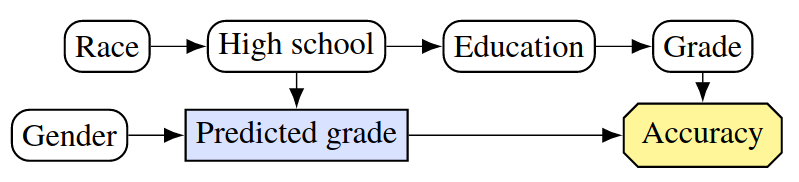
\includegraphics[width=0.5\textwidth]{pics/grade_prediction.png}}
% \caption{Source: \cite{everitt2021agent}. Here, discrimination is incentivized with respect to Race, but not incentivized with respect to Gender, because the edge from Gender is eliminated in $G^{min}$.}
% \label{grades}
% \end{figure}

% %%%%%%%%%%%%%%%%%%%%%%%%%%%%%%%%%%%%%%%%%%%%%%%%%%%%%%%%%%%%%%%%%%%%%%%%%%%%%%%%%%%%%%%

% \section{Research Plan and Preliminary Work}\label{plan}
% The first step will be to extend Theorem \ref{markov} to the Non-Markovian case: this is foundational for the following directions. (It seems trivial if confounding is not allowed on $D$, but then we wouldn't be able to say anything about the Berkeley admissions case).


% %%%%%%%%%%%%%%%%%%%%%%%%%%%%%%%  ^^ Transfered on 3/8  %%%%%%%%%%%%%%%%%%%%%%%%%%%%%%%


\section{First steps on non-markovian response incentives}

\newpage

\section{2/15 Synthesis of possible directions}
\begin{itemize}
  \item Non-markovian incentivized Cft-DE, Cft-IE, and Cft-SE [makes identification easier, while simultaneously measuring more accurately what policy makers care about: the effect of future policies]
  \item Incentivized fairness as a way to evidence reward-dependancies [mechanistic explanation of discrimination, to inform policy design]
  \item Decomposing VoC into direct/indirect VoC [??]
  \item (Providing a way to ensure CRL is fair)
  \item Decomposition of Introduced+Inentivised Total Variation [...]
  \item Prove that "CRL: opimizing counterfactual regret" will always be Cft-De, Cft-IE, or Cft-SE fair w.r.t some class of enviornments.
\end{itemize}


\section{2/15 Brainstorming}
\begin{itemize}
  \item I like the idea of "incentives allow us to prune"
  \item For example, I think we can even prune some Cft-DE's if they're not incentivised! (AKA d-seperated from utility given decision and observations).
  \item Perhaps a way to unify the two notations (fairness and CRL) is to say $X$ is the sensitive attribute, $D$ is the decision/policy node, and $Y$ is the reward. $C$ are the covariates, aka the inputs to $D$. $U$ is set of exogenous variables.
  \item Since pruning represents a strict reduction of the graph, it can only make identifiability easier. So it seems likely that there are some non-trivial classes of graphs for which the Cft-DE, Cft-IE, and Cft-SE effects were non-ID, they become ID in the reduced (incentivized) graphs!
  \item so there's "Incentivized counterfactual-fairness in non-markovian settings"
  \item as well as "direct/indirect VoC"
  \item Or, I could just do a "decompose the fairness effect into incetivized and non-incentivised"...since the non-incentivized effect should be null, if it's not it implies the policy is not optimal w.r.t. the reward function! I think this provides a testable implication of what the reward is! (For instance, it's easy to imagine that someone on the admissions commitee claims to only be optimizing the reward of future academic potential, but is actually optimizing a combined reward of this and a mysogonistic term). In short, this idea would provide an indicator for how much the effect (say Cft-DE for example) is attributable to the current reward function, under the assumption that the graphical model is correct).
  \item So how would this "decomposition w.r.t incentives" work? (especially considering the original decomposition was all about different paths). Well, the incentives effectively turn off some of the paths, so that only the variation of the remaining paths is measured. So it's very similar to the previous decomposition, where we subtracted off other paths to effectively shut them down - here, we just actually turn them off by removing those connections.
  \item So, I'm imagining that for each effect (Cft-DE, Cft-IE, and Cft-SE) we can further decompose it into two effects, which together combine (somehow) to form the total effect. 
  \item "Icv-E" and "Nicv-E"...or "I-Cft-DE, N-Cft-DE" for incentivized and non-incentivized, respectively...Or $Cft-DE\uparrow$ and $Cft-DE\downarrow$. Ohh I like the arrows!!!!
  \item So what problem does this insight solve that couldn't be solved before? 1. these subterms are more likely to be identifiable than the original term (you know, once we can do non-markov). 2. This provides testable implications of the reward (hopefully of the form "the reward is sufficient to explain the variation" and "the reward is neccesary to explain the variation") 3. The effect of automation on discrimination can be predicted (since the computers will have more clear rewards than humans, we can expect that the non-incentized variation will go to zero) 4. We can better inform policy design to break the problematic incentive links...
  \item in short, we're getting more clarity (about the reward, etc) by introducing more assumptions (about the reward). This is a tool that allows us to say how much a given reward assumption is enough to explain the variation.
  \item Revision on what it means if a non-incentivized effect is not null: I think it implies either 1. The agent is not rational, 2. The causal graph is inaccurate (for example, w.r.t the dependancies of the reward).
  \item Thus, if we assume the agent is rational, Then we can search among the reward-structures which minimizies the observed non-incentive unfairnesses. The reward structure which does so is most likely the true reward structure (assuming the rest of the graph is accurate, the data is infinite, etc). 
  \item In this way we can say that together the (data, enviornment assumptions) provide evidence about the reward structure.
  \item So, this would imply that we could provide empirical evidence about which graph in Figure 5 of https://arxiv.org/pdf/1902.09980.pdf is more plausible.
  \item ...Is this reasonable? Or does the fact that it would provide this distiction a red-flag that something's off? Let's run through the argument carefully.
  \begin{itemize}
    \item Let a fairness-effect measure $E$ be given. Fix everything about the causal graph except for the dependancies of the reward variable $Y$.
    \item Suppose that for a compatible $G_Y$ (with specified reward dependancies for $Y$) I have a procedure that allows me to find $E\uparrow$ and $E\downarrow$. 
    \item Suppose that I have a theorem that $E\uparrow$ and $E\downarrow$ combine again to form $E$ (in other words, they form a valid decomposition of $E$).
    \item Suppose the following conjecture holds: Assuming $G_Y$ represents the true structure which generated the data, and the agent is optimal w.r.t. $Y$, then $E\downarrow=0$.
    \item Then Conjecture: Assuming the agent was rational w.r.t optimizing $Y$, then $|E\downarrow|\ge0$ satisfies the metric axioms for how accurate the reward $Y$'s dependancies are.
    \item Epistemic status: I think it's likely a valid agument for simple (i.e. linear-standard) models. For non-parametric settings, it seems plausaible that there are edge cases which break the monotonicity needed for $E\downarrow$ to be a valid metric.
  \end{itemize}
\end{itemize}

"Understanding Agent Incentives using Causal Influence Diagrams" https://arxiv.org/pdf/1902.09980.pdf
\begin{itemize}
  \item They use the terms "observational incentive" and "interventional incentive". I think these terms will resonate more quickly with Bareinboim, so I'll use these!!
  \item It's probably fine for me to directly pull from this paper (I'll make sure I'm giving credit before I submit it, but for now just type fast)  
\end{itemize}


\section{Self-contained fairness drafting}

Notation notes (to maintain consistency with Elias’ lab):
\begin{itemize}
\item Decision node is X
\item Inputs to X are set C
\item Y is the reward
\item U refers to set of exogenous variables
\item Look at Justin’s “Experiments - Dynamic Treatment Regimes” slide 9 in lecture 4
\item The only difference is that in his setup, he’s minimizing cumulative regret over Y (over the training process), but incentives are maximizing expected value of Y (on that timestep) ... Maybe these are actually equivalent…
\item ...to show they're equivalent, all I need to do is show the two optimization problems are equivlent (have the same optima)
\end{itemize}

\begin{figure}[htbp]
\centerline{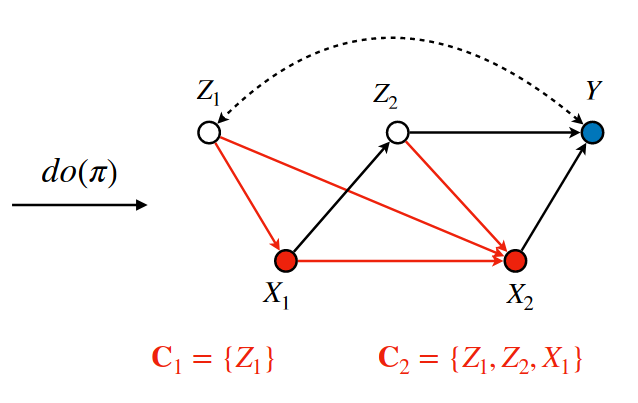
\includegraphics[width=0.5\textwidth]{pics/incentives_example_lecture_4.png}}
\caption{Example of a figure caption.}
\label{fig}
\end{figure}

Thoughts from youtube video about causal explanation formula
\begin{itemize}
  \item Note that in the COMPAS example, both $Y$ and $Y^*$ are present. So we can compute a reward based on this. $Y$ would be the decision node here, I think.
  \item \textbf{It is an open question how to do estimation of the variious CF effects in high-dimensional data!!}
  \item identification of the non-standard model, in parematrized settings. Linear, monotonic, etc. (monotonic might be a good fit for me? no idea really.)
  \item In the fairness setting, Y is the decision, and X is the sensitive attribute. There's often no utility node (which is why it conflicts with CRL notation).
\end{itemize}

\begin{figure}[htbp]
\centerline{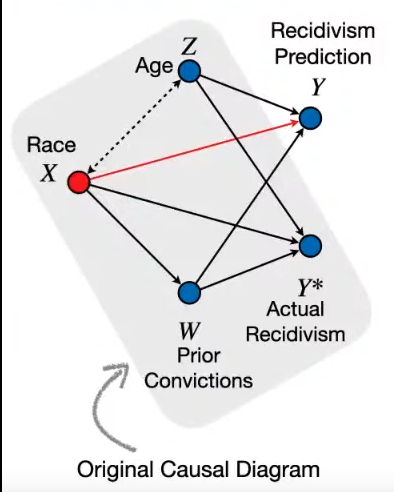
\includegraphics[width=0.3\textwidth]{pics/Discrimination_in_COMPAS.png}}
\caption{Example of a figure caption.}
\label{fig}
\end{figure}




\newpage
\section{CRL thoughts (outside work hours)}
\begin{itemize}
  \item While it might be nice to bring this into CRL (like in discussions of transportibility, etc) I don't want to brainstorm about it during work hours.
  \item Another idea: show that Counterfactual Regret (from the casino problem) induces less interventaional incentive than regular cumulative regret. (I think to be well-defined, this needs to be w.r.t to some set of variables which have interventional incentive.)
  \item again, using motivations like "ad-clicking" and "self-culfilling stock market predictions"
  \item Response incentives might also shed light on what changes in the enviornment the training will generalize to.
\end{itemize}







\newpage

\section{2/12 Bareinboim feedback}

"something that was not possible will be possible based on your insight X, Y, or Z."
\begin{itemize}
  \item This feels redundant, or like an applause light. What is he trying to get at?
  \item Maybe it's not that it constrains the space of "good research proposals" at all, but rather that expressing my proposals in this manner helps clarify the motivation behind the research. So it's a way to communicate better (but it doen't prohibit any research idea).
\end{itemize}

I'm very surprised that Elias thinks my "bounding causal effects over PDAGs" is difficult!
\begin{itemize}
  \item But that is the one he knows the best, so if he says it's not tractable, I do believe him. 
  \item I \emph{think} this means that I should not focus on this proposal, just the other 2...
  \item...Wait. All he really said is that I haven't yet offered any insights of my own about how it can be solved. Which is accurate. So, do I have any such insights?
\end{itemize}

Structural constraints inferred from an identification function
\begin{itemize}
  \item He says it's not clearly articulated yet, which I already knew.
  \item I do have a more clear example I can provide him.
  \item Personally, I'm more concerned about how to connect it to neural networks...
\end{itemize}

Incentivsed Unfairness
\begin{itemize}
  \item He says it needs to be self-contained.
\end{itemize}

\section{2/11 Blei feedback}
\begin{itemize}
  \item Not as familiar with non-markovian systems, but open to it.
  \item \textbf{Ultimately we want the whole pipeline: so I need data/code, as a necessity for this project.}
\end{itemize}

\newpage
\section{Structural constraints inferred from an identification function}
\subsection{Backdoor example}
I think the next step for Elias is to come up with a baby example. This will help me reach out to the AIS person as well. And, it might make it easier to identify how to make it connect to NNs (which all three care about).

Suppose $G$ has a backdoor-admissible set $Z$ for the causal effect of $X$ on $Y$. Then 
\[
P(Y|do(X=x)) := f(P(V)) = \sum_z P(Y|x,z)P(z)
\]

Let's say you hand me an algebraic function $f(P(V)) = \sum_z P(Y|x,z)P(z)$. I'll take one look at it and (because it's expressed algebraically) recognize it as the backdoor formula, and conclude that $Z$ must be admissable for adjustment. Consequently, I know that the set $\mathbb{G}_f$ of causal diagrams $G$ which admit $f$ can only be ones satisfying the backdoor criterion w.r.t. $\{X,Y,Z\}$. [make this a 3-variable example, to make even more concrete. Starts with all possible configurations, eliminates the ones that don't fit]

Now, let's take a step back, away from full agebraic knowledge of $f$. Say I have a numeric representation of $f$, mapping the joint distribution $P(V)$ to the distribution $P(Y|do(X))$. By running some numerical differentiation, I know that the only non-zero partial derivatives of $f$ are
\begin{align*}
& \frac{\partial f}{\partial P(Y|x,z)} \neq 0\\
& \frac{\partial f}{\partial P(z)} \neq 0 
\end{align*}
for at least some values of $z$. What can be said about $\mathbb{G}_f$? Well, I know $f$ depends only on the probabilites $P(Y|x,z)$ and $P(z)$.

[...Uh oh. What if the fact that these partials are nonzero, implies others are as well?? Since these probabilites have relationships with the other conditional probabilities, it seems like that might happen. If it does, then how do I conclude that $f$ depends only on these probabilities?]

[I don't like the idea of doing a symbolic regression to get the formula back - I expect it to be way too sensitive to pertubation.]

\subsection{Neccessary and Sufficient criteria}
What restrictions does a causal diagram $G$ impose on the function $f$? Or vice versa?


\subsection{2/13 Assessment}
\begin{itemize}
  \item I think the fact that there's too much new here. I'm having to wade through a lot of uncertainty, etc.
  \item Perhaps some (more applied) variation of this proposal could work for Blei. But I don't think it's going to work well for Bareinboim. I tentatively lean towards dropping it.
\end{itemize}

\newpage
\section{Bounding Causal effects over PDAGs}
\subsection{10 minutes thinking of my own insights}
So, how would I go about bouding causal effects over PDAGs? I'll give it 10 minutes of thought, and let it go if I can't think of anything at that point.

Well, I would first try to mimic Justin's approach. 1. I think every graph implies natural bounds? Check this. 2. Apply these natural bounds to every graph in the equivalence class, and 3. optimize over these bounds. 

Perhaps some graphs will tend to be the ones that have the most extreme bounds? If we knew which ones, we could just focus on those...That would be a ssignificant insight.

Let's run with that idea. Can I think of any reason why some graphs would for sure have more extreme bounds than other ones?

Experimentally, we could just do a Bayesian update over all of them, and Thompson-sampling style focus on the ones which are more likely to make the bound worse...

Is there some kind of dual to the problem? That would be an intersting insight...I know I learned about duals for linear programming, is there something similar for polynomial programming? I'll look it up quick: (didn't find any)

\subsection{Current Assessment}
As of right now, I have no new insights to contribute. After spending 10 minutes attempting, my gut isn't feeling terribly optimistic about finding low-hanging fruit. I don't think I have enough evidence to overcome Elias' prior on how difficult this will be.

So, for now I will not actively think about this problem any longer. Only if I get spontaneous insights before the end of Monday.



\newpage

\begin{itemize}
  \item filler
\end{itemize}

\[
\frac{\partial f}{\partial g}
\]

\end{document}
